\section{Prophets of Electrum}

\begin{wrapfigure}{rt}{.3\textwidth}
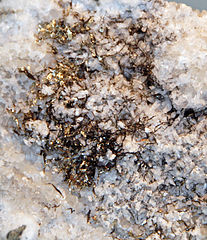
\includegraphics[width=.25\textwidth]{207px-Electrum_on_quartz.jpg}
\end{wrapfigure}

\begin{quotex}
Consciousness in man is pre-eminently intellect. It might have been, it ought, so it seems, to have been also intuition. Intuition and intellect represent two opposite directions of the work of consciousness: intuition goes in the very direction of life, intellect goes in the inverse direction, and thus finds itself naturally in accordance with the movement of matter. A complete and perfect humanity would be that in which these two forms of conscious activity should attain their full development.
\flright{\textsc{Henri Bergson}, \emph{Creative Evolution}}

Here is the difference between the nature of intelligence and that of intuition of faith, between the principle of autumn and that of spring. The former is \emph{understanding of that which is}; the latter is
\emph{participation in the becoming of that which is to be.}
\flright{\textsc{Meditations on the Tarot}, \emph{Letter XVIII The Moon}}
\end{quotex}

One of the tasks of Hermetism is to accomplish the alliance of intelligence and the intuition of faith --- the alchemical marriage of the moon and the sun. Another way to put it is to obtain the alloy of silver and gold, which is called Electrum. Although some have come close to this ideal, it is a task still incomplete. Several thinkers have come close; these we will call the \textbf{Prophets of Electrum}.

At the top of those prophets is \textbf{Saint Thomas Aquinas} whose thought is silvered gold. More common is gilded silver as expressed by Origen, Dionysius the Areopagite, Jacob Boehme\footnote{See Section \ref{sec:ChristianGnosis} in this book.}, Louis Claude de Saint-Martin\footnote{See Section \ref{sec:HiddenTradition} in this book.}, Vladimir Solovyov, Nicolas Berdyaev\footnote{\url{https://gornahoor.net/?s=Berdyaev}}, Henri Bergson, and Pierre Teilhard de Chardin.

The importance of Thomas Aquinas cannot be overestimated, even for Hermetists. The raison d'être of scholasticism is the union of faith and intelligence. Following his conversion to Catholicism, Tomberg wrote his graduate thesis on International Law from a Thomist perspective, so he was quite familiar with Thomas's work. In particular, he referred to Thomas's mystical experience near the end of his earthly life:

\begin{quotex}
On the feast of St. Nicholas, 1273, Aquinas was celebrating Mass when he received a revelation that so affected him that he wrote and dictated no more, leaving his great work the Summa Theologiae unfinished. To Brother Reginald's (his secretary and friend) expostulations he replied, ``The end of my labors has come. All that I have written appears to be as so much straw after the things that have been revealed to me.'' When later asked by Reginald to return to writing, Aquinas said, ``I can write no more. I have seen things that make my writings like straw.''
\flright{\textsc{Alban Butler}, \emph{Lives of the Saints}}
\end{quotex}


But that experience was not a rejection of his purely intellectual work, but rather its fulfilment. Thomism is the combustible that, when enflamed, gives rise to contemplation:

\begin{quotex}
\textbf{St. Thomas Aquinas} was not the only one. Just as he arrived at contemplation through scholastic reasoning, so did the peak of the scholastic wave reach gnosis \emph{mystique}, that is to say, intuition or the state of union of faith and intelligence, which is the aim of scholasticism. \textbf{Meister Eckhart}, \textbf{Ruysbroeck}, the Admirable Doctor, \textbf{St. John of the Cross} are in fact spirits amongst whom you will search in vain for a spirit of opposition to scholasticism. For them also it was true that scholasticism was ``like straw'', but they knew at the same time from their own experience that this straw is an excellent combustible. They certainly surpassed scholasticism, but after having attained its aim. For the aim of scholastic effort is contemplation, and it is gnosis \emph{mystique} which is the fruit of the scholastic tree.
\flright{\textsc{Valentin Tomberg}, \emph{Letter XIX The Sun}}
\end{quotex}


Some of the persons mentioned are controversial from the strictly metaphysical point of view. However, Hermetism is not concerned with dialectics but rather with mining their insights. There faults are acknowledged, but left aside. That is why they are gilded silver.

Pierre Teilhard de Chardin is the scientist who approaches the ideal. He restored the subjective element to scientific objectivity, in the claim that there is an ``inside'' as well as an ``outside'' to everything. Any complete understanding of the world process needs to take that into account. Teilhard advanced the ``postulate of the pre-existence of a prototype for all beings, which is the ultimate as well as the effective cause of the whole process of evolution, and this postulate alone tenders evolution intelligible.''. Isn't that essentially Platonism, where the divine ideas are expressing themselves in time?

Although Tomberg writes extensively about Henri Bergson, I'd like to add a little more background. Finally, I'll conclude with the influence of Vladimir Solovyov which, I believe, provides a view into Tomberg's motivation.

\paragraph{Henri Bergson}


\begin{quotex} There is a centre from which worlds shoot out like rockets in a fireworks display---provided, however, that I do not present this centre as a thing, but as a continuity of shooting out. God thus defined, has nothing of the already made; He is unceasing life, action, freedom. Creation, so conceived, is not a mystery; we experience it in ourselves when we act freely.
\flright{\textsc{Henri Bergson}, \emph{Creative Evolution}}
\end{quotex}


Henri Bergson's philosophy was born in the atmosphere of French spiritualism, a form of idealism prominent in Italy and France at the time. One influence, for example, was \textbf{Emile Boutroux} who in the Contingency of Physical Laws, claimed that life, feeling, and freewill need to be part of any understanding of Physical Laws. He rejected determinism, and instead claimed that natural laws as a sort of ``habit'' of things: what originally was also able to be a free act, in repeating itself, automatizes, and mechanizes itself and ends up appearing to be a necessity. A fortiori, this applies to human beings, who cannot be determined by environment, race, etc.

Bergson married a cousin of Marcel Proust and his brother-in-law was Samuel Liddell MacGregor Mathers, a founder of the \emph{Hermetic Order of the Golden Dawn}. Although born Jewish, Bergson felt closer to Catholicism, which he regarded as the fulfilment of Judaism. He never officially converted, however, because of the rise of National Socialism.

Although from a strictly logical point of view, his philosophical system can be refuted. The Church even banned his books. Rene Guenon, too, was critical of Bergson. However, that is not the Hermetic reading of Bergson, which is more concerned with Bergson's insights than its logical presentation. Any useful critique of his thought would have to advance the alliance of intelligence and intuition. The standard critiques remain on one or the other side of that alliance, and therefore fall short of what is necessary.

In Bergson's view, the intellect treats matter as inert, and is unable to discern the life that animates it. It chops Being up into pieces, so that ``whatever is fluid in the real will escape it''. We see this starkly in the abortion debate: science cannot determine when ``life begins in the womb''. The intelligent course of action in this case would be to admit that shortcoming of ``science'' and rely on one's intuition. That seldom happens, so the modern world loves death and sterility.

\paragraph{Solovyov and Egyptian Theosophy}


In a footnote to Lecture Six of \emph{Divine Humanity}, Vladimir Solovyov informs us:

\begin{quotex}
Although the close inner connection between Alexandrian theosophy and the Christian doctrine is one of the firmly established theses of Western scholarship, for one reason or another, this perfectly correct thesis does not enjoy common acknowledgement in our theological literature. Therefore, I consider it necessary to devote to this question a special appendix at the end of these lectures, where I will touch upon the significance of the native Egyptian theosophy (the revelations of Thoth or Hermes Trismegistus) in its relation to both the doctrines mentioned.
\end{quotex}


Unfortunately, this pregnant quotation is the theological equivalent of Fermat's Last Theorem, since the promised appendix was never published. This section will try to begin the proof. First of all, the two doctrines in question are the dogmas of the Logos and the Trinity. These doctrines were developed metaphysically by Egyptian Neoplatonists from Philo to Plotinus independent of Christian revelation. What Christianity brought was the revelation that this divine life appeared as a fact, as an historical reality. Only later was this fact connected to Neoplatonic metaphysics. Now we see how Solovyov became a prophet of Electrum, uniting the intuition of faith with the intelligence of metaphysics.

So, how does this relate to Valentin Tomberg? In a talk \textit{Inner Impulses of Evolution}\footnote{\url{https://web.archive.org/web/20251212133332/https://rsarchive.org/Lectures/GA171/English/AP1984/InnImp_index.html}}, Rudolf Steiner mentions Solovyov in relation to \textbf{Ernest Renan} and \textbf{David Strauss}. Renan wrote a \emph{Life of Christ} that presumes that Jesus was simply a man living in Palestine at a certain historical time. Hence, he strips out all supernatural and miraculous elements from the Gospels.

Strauss' \emph{Life of Christ}, on the other hand, wrote from the perspective of Jesus' followers. The miracles, for example, were mythical, i.e., creations of the early Christians to express their developing conception of Jesus. Since Strauss was a Hegelian, he did not deny spiritual reality in itself. Steiner interprets Strauss like this:

\begin{quotex}
As Strauss sees it, in the course of mankind's earthly development, from the times of the first beginnings of the earth to its final end, mankind has and always will have a higher power in it than the merely external power that develops on the physical plane. A power runs right through mankind that will forever address itself to the super-earthly; this super-earthly finds expression in myths. We know that man bears something supersensible within him that seeks to find expression in myth since it cannot be expressed in external physical science. Thus, Strauss does not see Jesus in the single individual, but rather the Christ in all men.
\end{quotex}


Solovyov, on the other hand, focuses on Christ rather than Jesus, but on Christ as a living being, not as an abstract idea. Steiner describes Solovyov, perhaps with some exaggeration:

\begin{quotex}
When we come to Soloviev, behold, Jesus is no more, but only the Christ. Nevertheless, it is the Christ conceived as living. Not working in men as an idea, with the consequence that its power is transformed in him into a myth, but rather working as a living Being who has no body, is always and ever present among men, and is, in effect, positively responsible for the external organization of human life, the founder of the social order.
\end{quotex}


Steiner's lecture made quite an impression on the young Tomberg, who was inspired to study Solovyov in depth. Tomberg describes that encounter:

\begin{quotex}
A result was the conviction that this author had never encountered a work written before the time of Rudolf Steiner that contained such a profound concept of the nature and mission of Jesus Christ, a view presented against the background of cosmic history.
\end{quotex}


The obvious question is how did Solovyov arrive at such a deep understanding. This perplexed Tomberg, since Solovyov certainly did not argue himself into his understanding, despite presenting his understanding in a logical way to others. Solovyov does mention three divine experiences of Sophia, including one in the Egyptian desert. We don't know exactly what he was doing in Egypt, but we do know that Solovyov had become quite familiar with both the Kabbalah and Hermetism. He regarded Paracelsus, Boehme, and Emmanuel Swedenborg as ``substantial individuals''. He was also familiar with Johann Gichtel, so he would have known of Gichtel's correspondence of the chakras with the planets\footnote{\url{https://gornahoor.net/?p=16036}}.

So we can read the Letters on the Tarot as the promised appendix to \emph{Divine Humanity}. Tomberg explains in the Forward:


\begin{quotex}
These Letters are intended only to serve, to sustain, and to support the Hermetic tradition --- from its first appearance in the epoch of \textbf{Hermes Trismegistus}, lost in the remoteness of antiquity and become legendary.
\end{quotex}



\flrightit{Posted on 2022-04-21 by Cologero}

\begin{center}* * *\end{center}

\begin{footnotesize}
\begin{sffamily}

\texttt{Carol on 2022-04-22 at 15:22 said:}

Hello, I don't usually comment on blogs, but I have been reading here for some time now and would like to express my appreciation for your posts!

I am a 58 year old American woman with very little formal education... but I have tremendous admiration for those who, being highly educated, combine their intellectual skills with spiritual pursuits.

I particularly enjoy posts such as this current one, as I have not got the mental fortitude to read entire works by such authors as you `discuss' here.

But your writing is very `accessible' to my understanding and thus, very helpful toward the limitations of my intellect in my pursuit of spiritual materials for contemplation.

Anyway, I just wanted you to know that you have a reader who is very grateful for your efforts!!!

\hfill

\end{sffamily}
\end{footnotesize}

